% ======================================================================
\section{The status quo, privilege, and individually rational exploration}\label{sec:sq}
% ======================================================================

So far every loss has been measured against $\astar$ or against a person's own favourite policy. People who object to a reform usually measure against something else: the policy already in force. This section adds a status quo and asks what can be learned without making anyone worse off than under it.

\subsection{The status quo as a baseline}

Let one arm, $a_0\neq\astar$, be the \emph{status quo}. It has been in force for a long time, so its means $\mu_{\cdot,a_0}$ are known. Person $i$'s gain from the planner's choices, relative to keeping the status quo, is
\[
  G_i(T)=\sum_{t=1}^T(\mu_{i,a_t}-\mu_{i,a_0})=T\,(\mu_{i,\astar}-\mu_{i,a_0})-R_i(T).
\]
The first term is person $i$'s stake in reform. It is linear in $T$ and it can be negative: the utilitarian optimum is a potential-compensation improvement on the status quo, in the sense of Kaldor and Hicks, and need not be a Pareto improvement.

\begin{definition}[Privilege]\label{def:privilege}
Person $i$'s \emph{status-quo regret} is $\rho^0_i=m_i-\mu_{i,a_0}$, the amount per round by which the status quo falls short of person $i$'s favourite policy. Person $i$ is \emph{more privileged} than person $j$ if $\rho^0_i<\rho^0_j$.
\end{definition}

Privilege in this sense is a fact about a person and a policy menu, not about the person alone. A person with $\rho^0_i=0$ has their favourite policy already. For them every trial of anything else is a loss, and no amount of redirected exploration can change that; this is \cref{cor:irreducible} with the baseline moved from $\astar$ to $a_0$. A person with large $\rho^0_i$ has the most to gain from some reform, though not necessarily from the one that is best in total.

Two remarks connect the definition to exploration.

\emph{Exploration is progressive in expectation.} Suppose that, before anything else has been tried, the planner regards the untried arms as exchangeable, and let $\bar m_i$ be the reward it expects person $i$ to get from any one of them. Trying an untried arm for one round then changes person $i$'s expected reward by $\bar m_i-\mu_{i,a_0}$. This is negative exactly for the people whom the status quo places above what they could expect from an arbitrary alternative, and it falls one for one as $\mu_{i,a_0}$ rises. So the people best served by the status quo expect to pay for experiments, and the people worst served expect to gain from them.

\emph{Not exploring is not neutral.} A planner that never leaves $a_0$ has $G_i(T)=0$ for everyone and imposes a loss of $T(\mu_{i,\astar}-\mu_{i,a_0})$ on everyone with a positive stake in reform. The status quo is an arm, and keeping it has a regret vector like any other choice \citep{meyer2015}.

\begin{example}[A status quo]\label{ex:sq}
Add to \cref{ex:blog} a status quo $a_0$ with rewards $(1.2,\,1.2,\,0.2)$, so $W(a_0)=2.6$. The status-quo regrets are $\rho^0=(0.3,\,0.3,\,0.8)$: persons 1 and 2 are the more privileged. Moving to $\astar$ raises welfare by $0.4$ per round, costs persons 1 and 2 $0.2$ each, and gives person 3 $0.8$. A planner that learns $\astar$ in the standard way must also rule out $a_0$ ($\Delta_{a_0}=0.4$, $\cmin_{a_0}=37.5$); its learning burdens are $(-306,\,-306,\,691)$ per unit of $\log T$ and total regret is $79\log T$.
\end{example}

\subsection{Individual rationality}

A constraint that protects each person relative to the status quo has to be stated per round, because a planner that is allowed to make a person worse off now on the promise of later gains is asking for exactly the trust that is in question.

\begin{definition}[Individually rational planner]\label{def:ir}
Let $p_t$ be the distribution from which the planner draws $a_t$, given the history. For $\alpha\ge0$ and $\delta\in(0,1)$, the planner is \emph{$\alpha$-individually rational with confidence $1-\delta$} on a class of instances if, on every instance in the class,
\[
  \Prob\big(\,(\mu p_t)_i\ \ge\ \mu_{i,a_0}-\alpha\ \text{ for all } i \text{ and all } t\,\big)\ \ge\ 1-\delta .
\]
\end{definition}

The tolerance $\alpha$ is the expected loss per round, relative to the status quo, that each person can be asked to accept. It may differ between people; we take it equal to keep the notation light. We work on the class $\Env_L$ of instances that share the known status-quo means and satisfy $|\mu_{i,a}-\mu_{i,a_0}|\le L$ for all $i$ and $a$, for a known $L>0$. Without some such bound a planner knows nothing at all about an untried arm.

\begin{proposition}[No free trial]\label{prop:nofree}
If a planner is $0$-individually rational with confidence $1-\delta$ on $\Env_L$, then on every instance in $\Env_L$ the probability that it ever plays an arm other than $a_0$ is at most $\delta$.
\end{proposition}

\begin{proof}
Let $\tau$ be the first round in which $p_\tau(a_0)<1$, with $\tau=\infty$ if there is none. Before $\tau$ only $a_0$ has been played, and the law of its observations is the same on every instance in $\Env_L$, so the probability of $\{\tau<\infty\}$ is the same on every instance. Let $\nu^-$ be the instance with $\mu_{i,a}=\mu_{i,a_0}-L$ for all $i$ and all $a\neq a_0$; it lies in $\Env_L$ and $a_0$ is its unique welfare maximiser. On $\nu^-$, if $\tau<\infty$ then $(\mu p_\tau)_i=\mu_{i,a_0}-L(1-p_\tau(a_0))<\mu_{i,a_0}$, which violates the constraint. So $\{\tau<\infty\}$ has probability at most $\delta$ on $\nu^-$, hence on every instance, and the planner cannot play another arm unless $\tau<\infty$.
\end{proof}

So a collective that will not accept any expected loss for anyone, even for one round, cannot learn anything. Experimenting on a public arm requires some tolerance, and $\alpha$ is where that requirement is made explicit.

\subsection{What an individually rational planner should aim at}

With the means known, the best a planner can do under the constraint is the time-share
\[
  p^\star_\alpha\in\arg\max_p\Big\{\mathbf 1^\top\mu p:\ \mu p\ge\mu_{\cdot,a_0}-\alpha\mathbf 1,\ p\ge0,\ \mathbf 1^\top p=1\Big\},
\]
a linear program, feasible because $p=e_{a_0}$ satisfies it. Its value $W_\alpha$ is concave and nondecreasing in $\alpha$. The optimal dual variable $\lambda_i$ on person $i$'s constraint is the welfare the collective would gain per round from one more unit of tolerance from person $i$. It is zero for anyone whose constraint is slack, and positive only for people whose protection is holding the collective back: it is the price of person $i$'s veto. In general the solution is a time-share and not a single policy, so individual rationality leads to \cref{sec:sharing} whether or not fairness was the aim.

\begin{proposition}[When unanimity blocks everything]\label{prop:weights}
The following are equivalent: (a) no time-share gives every person strictly more than the status quo; (b) there are welfare weights $w\ge0$, $w\neq0$, under which the status quo maximises $\sum_iw_i\mu_{i,a}$ over arms.
\end{proposition}

\begin{proof}
Let $A=\mu-\mu_{\cdot,a_0}\mathbf 1^\top\in\R^{N\times K}$. Statement (a) fails if and only if there is $p\ge0$ with $Ap>0$ (normalise $p$ to sum to one; $p=0$ is excluded by the strict inequality). By \cref{lem:alt} applied to $M=-A$, this is the alternative to the existence of $w\ge0$, $w\neq0$, with $w^\top A\le0$, which says $\sum_iw_i\mu_{i,a}\le\sum_iw_i\mu_{i,a_0}$ for every arm $a$.
\end{proof}

When such weights exist they are a second description of privilege: they say whose interests the status quo is optimal for. A status quo that no unanimous reform can improve is one that is exactly right for somebody's weighting of the population, and the further those weights are from equal, the more unequal the protection that unanimity gives.

\begin{example}\label{ex:ir}
In \cref{ex:sq} no weights rationalise $a_0$: they would need $w_3\ge w_1+w_2$ for $a_0$ to beat $b$ and $w_3\le(w_1+w_2)/4$ for it to beat $\astar$. So a unanimous improvement exists. The best one is $p^\star_0$: $\astar$ for $60\%$ of the time and $b$ for $40\%$, with rewards $(1.2,\,1.2,\,0.56)$ and welfare $2.96$ (\cref{fig:sharing}). Persons 1 and 2 are held exactly at their status-quo level and person 3 gains $0.36$. The collective gives up $0.04$ per round relative to $\astar$, and the price of the protection is $\lambda_1+\lambda_2=0.2$: each unit of tolerance from persons 1 and 2 together would buy $0.2$ of welfare. With $\alpha=0.05$ the target is $70\%$ $\astar$ and $30\%$ $b$, with welfare $2.97$.
\end{example}

\begin{figure}[t]\centering
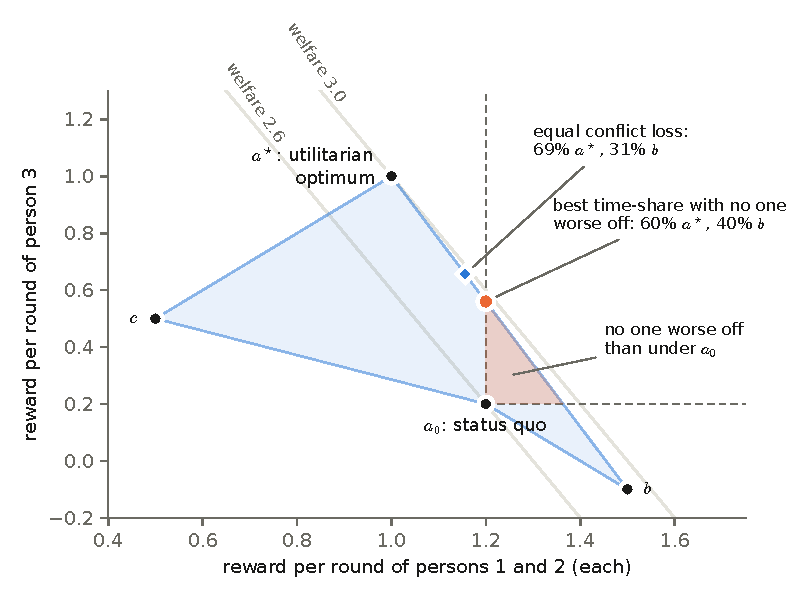
\includegraphics[width=0.72\linewidth]{figures/fig_sharing.pdf}
\caption{\Cref{ex:sq}: the reward vectors that time-sharing can reach (shaded blue), projected on persons 1 and 2 (identical) and person 3. The status quo $a_0$ lies inside the set, so some time-shares make everyone better off (shaded orange). The best of these in total is $60\%$ $\astar$, $40\%$ $b$. The diamond is the time-share with the smallest largest conflict loss (\cref{prop:share}). Grey lines join points of equal welfare.}
\label{fig:sharing}
\end{figure}

On random instances, with the status quo drawn at random among the arms other than $\astar$, unanimity blocks everything most of the time, and nearly always once there are many people and few policies (\cref{tab:ir}). A tolerance of $\alpha=0.1$, a tenth of the standard deviation of a reward, recovers a modest part of the available gain. Pure policy choice gives few Pareto improvements; the rest have to come from tolerance or from transfers.

\begin{table}[h]\centering\small
\begin{tabular}{rrcc}
\toprule
$N$ & $K$ & no unanimous improvement exists & median share of the gain recovered with $\alpha=0.1$\\
\midrule
3 & 3 & 64\% & 30\%\\
5 & 4 & 79\% & 14\%\\
10 & 5 & 98\% & 7\%\\
20 & 8 & 100\% & 5\%\\
\bottomrule
\end{tabular}
\caption{400 random instances per row ($\mu_{i,a}\sim\mathcal N(0,1)$ i.i.d.), status quo uniform among arms other than $\astar$. Second column: $W_0=W(a_0)$. Third column: median of $(W_{0.1}-W(a_0))/(W(\astar)-W(a_0))$.}
\label{tab:ir}
\end{table}

\paragraph{Transfers.} If rewards could be moved between people, the utilitarian optimum could be made individually rational by paying the losers: in \cref{ex:sq}, $0.4$ per round from person 3 to persons 1 and 2. In a model of committee experimentation with strategic voters, \citet{anesi2021} find that a small amount of redistribution restores efficient experimentation where veto rights do not. \Cref{sec:comp} sets up compensation as an institution and compares it with the floors of this section.

\subsection{A planner that is individually rational by construction}

The planner observes every person's reward. For an arm $a\neq a_0$ that has been played $n$ times, let $\hat\mu_{i,a}$ be person $i$'s sample mean and set
\begin{align*}
  r_n&=\sqrt{\frac{2}{n}\log\frac{4NK\,n(n+1)}{\delta}}, &
  \ell_{i,a}&=\max\{\hat\mu_{i,a}-s_ir_n,\ \mu_{i,a_0}-L\},\\
  && U_a&=\min\Big\{\textstyle\sum_i\hat\mu_{i,a}+\sigma r_n,\ W(a_0)+NL\Big\},
\end{align*}
where $s_i^2=\Sigma_{ii}$. For an untried arm, $\ell_{i,a}=\mu_{i,a_0}-L$ and $U_a=W(a_0)+NL$; for the status quo both are exact. In round $t$ the planner computes
\begin{itemize}[leftmargin=*,itemsep=1pt]
  \item an \emph{exploiting} time-share $q_t$, which maximises $\sum_ap_aU_a$ subject to $\sum_ap_a\ell_{i,a}\ge\mu_{i,a_0}-\alpha$ for all $i$;
  \item an \emph{exploring} time-share $e_t$, which maximises the smallest weight on any arm other than $a_0$, subject to the same constraints;
\end{itemize}
and draws $a_t$ from $p_t=(1-\gamma_t)q_t+\gamma_te_t$ with $\gamma_t=t^{-1/3}$. It is optimistic about welfare and pessimistic about each person's reward, as in conservative and safe bandits \citep{wu2016,amani2019,moradipari2020}, with one floor per person in place of one for the total.

\begin{proposition}[Safety]\label{prop:safe}
On $\Env_L$ this planner is $\alpha$-individually rational with confidence $1-\delta$.
\end{proposition}

\begin{proof}
For fixed $i$, $a$ and $n$, the mean of the first $n$ observations of person $i$ under arm $a$ is Gaussian with mean $\mu_{i,a}$ and variance $s_i^2/n$, so $\hat\mu_{i,a}-s_ir_n>\mu_{i,a}$ with probability at most $\exp(-nr_n^2/2)=\delta/(4NKn(n+1))$. Summing over $n\ge1$, over $N$ people and over at most $K$ arms gives probability at most $\delta/4$ that $\ell_{i,a}>\mu_{i,a}$ ever holds for some $i$ and $a$ (the truncation at $\mu_{i,a_0}-L$ is valid on $\Env_L$). Outside that event, $\ell_{i,a}\le\mu_{i,a}$ throughout, and both $q_t$ and $e_t$ satisfy $\sum_ap_a\mu_{i,a}\ge\sum_ap_a\ell_{i,a}\ge\mu_{i,a_0}-\alpha$. The constraint is linear, so the mixture $p_t$ satisfies it too.
\end{proof}

The exploring share is what makes the planner learn. Before anything has been tried it puts weight $\alpha/((K-1)L)$ on each untried arm: the tolerance, divided by the worst that could happen. Optimism alone is not enough here. If a known arm pays more welfare per unit of tolerance used than an untried arm could under the most optimistic assumption, the exploiting share spends the whole tolerance on the known arm and never tries the other.

The planner's regret against its own target is of order $T^{2/3}$.

\begin{proposition}[Regret]\label{prop:regret}
Let $\alpha\le L$, and let $W_\alpha$ be the welfare of $p^\star_\alpha$. On every instance in $\Env_L$, with probability at least $1-2\delta$, for all $T$,
\[
  \sum_{t=1}^T\big(W_\alpha-W(p_t)\big)\ \le\ C_0+C_1\,T^{2/3}\sqrt{\log\frac{4NKT^2}{\delta}},
\]
\[
  C_1=3NL+6\Big(\frac{s_{\max}(W_\alpha-W(a_0))}{\alpha}+\sigma\Big)\sqrt{\frac{(K-1)L}{\alpha}},
\]
where $s_{\max}=\max_is_i$ and $C_0$ does not depend on $T$.
\end{proposition}

\begin{proof}
Let $\mathcal G$ be the event that $|\hat\mu_{i,a}-\mu_{i,a}|\le s_ir_n$ and $|\sum_i\hat\mu_{i,a}-W(a)|\le\sigma r_n$ for all $i$, all $a\neq a_0$ and all sample sizes $n$. As in \cref{prop:safe}, each of these $2(N+1)K$ families of events fails for some $n$ with probability at most $\delta/(4NK)$, so $\Prob(\mathcal G)\ge1-\delta$. On $\mathcal G$ every $p_t$ satisfies the true constraints, so $W(p_t)\le W_\alpha$ and each term of the sum lies in $[0,2NL]$.

\emph{Every arm is tried often.} Let $\eta=\alpha/((K-1)L)$. The time-share with weight $\eta$ on each arm other than $a_0$ and the rest on $a_0$ satisfies the pessimistic constraints whatever the estimates, because $\ell_{i,a}\ge\mu_{i,a_0}-L$. So $e_t(a)\ge\eta$ and $p_t(a)\ge\eta\gamma_t$ for every $a\neq a_0$. The count $n_a(t)$ minus $\sum_{s\le t}p_s(a)$ is a martingale with increments bounded by one, so by the Azuma--Hoeffding inequality and a union bound over $a$ and $t$, with probability at least $1-\delta$,
\[
  n_a(t)\ \ge\ \eta\sum_{s\le t}s^{-1/3}-\sqrt{2t\log\frac{Kt(t+1)}{\delta}}\quad\text{for all } a\neq a_0 \text{ and all } t.
\]
Since $\sum_{s\le t}s^{-1/3}\ge\tfrac32(t^{2/3}-1)$ and the square root is of order $t^{1/2}$ up to a logarithm, there is $t_0$, depending on $\eta$, $K$ and $\delta$ only, with $n_a(t)\ge\tfrac12\eta\,t^{2/3}$ for all $t\ge t_0$. Call this event $\mathcal H$.

\emph{The exploiting share is nearly optimal.} Work on $\mathcal G\cap\mathcal H$ at a round $t>t_0$, and let $r=r_n$ at $n=\tfrac12\eta(t-1)^{2/3}$, which bounds the radius of every arm. On $\mathcal G$, $\ell_{i,a}\ge\mu_{i,a}-2s_ir$ and $W(a)\le U_a\le W(a)+2\sigma r$. Let $\theta=2s_{\max}r/\alpha$, and enlarge $t_0$ if necessary so that $\theta\le1$. The time-share $p'=(1-\theta)p^\star_\alpha+\theta e_{a_0}$ satisfies the pessimistic constraints:
\[
  \textstyle\sum_ap'_a\ell_{i,a}\ \ge\ \sum_ap'_a\mu_{i,a}-2s_ir\ \ge\ (1-\theta)(\mu_{i,a_0}-\alpha)+\theta\mu_{i,a_0}-2s_ir\ \ge\ \mu_{i,a_0}-\alpha .
\]
Since $q_t$ maximises $\sum_ap_aU_a$ over such time-shares, $\sum_aq_{t,a}U_a\ge\sum_ap'_aU_a\ge W(p')=W_\alpha-\theta(W_\alpha-W(a_0))$, and $W(q_t)\ge\sum_aq_{t,a}U_a-2\sigma r$. Hence
\[
  W_\alpha-W(q_t)\ \le\ 2r\Big(\frac{s_{\max}(W_\alpha-W(a_0))}{\alpha}+\sigma\Big).
\]

\emph{Summing.} $W_\alpha-W(p_t)\le(W_\alpha-W(q_t))+2NL\gamma_t$. With $r\le2\sqrt{\log(4NKT^2/\delta)/\eta}\,(t-1)^{-1/3}$ for $t\le T$, and $\sum_{t\le T}t^{-1/3}\le\tfrac32T^{2/3}$, the rounds after $t_0$ contribute at most $C_1T^{2/3}\sqrt{\log(4NKT^2/\delta)}$ up to an additive constant, and the rounds up to $t_0$ at most $2NLt_0$.
\end{proof}

The constants are not optimised, and the analyses of safe linear bandits suggest that a rate of $\sqrt T$ may be attainable with a better schedule. The form of $C_1$ is informative all the same: it grows like $\alpha^{-3/2}$, so a tight tolerance is paid for in slow learning. \Cref{sec:comp} shows that part of this is unavoidable.

\paragraph{Simulation.} \Cref{fig:planner} runs the planner on \cref{ex:sq} with $\alpha=0.05$, $L=1$ and $\delta=0.05$, against UCB on the welfare signal. Over 20 runs of $2\times10^5$ rounds the smallest per-round margin $(\mu p_t)_i-\mu_{i,a_0}$ was $-0.033$, inside the floor of $-0.05$. At the end the planner's time-share averaged $64\%$ $\astar$ and $36\%$ $b$, against a target of $70\%$ and $30\%$; persons 1 and 2 were within $0.01$ of their status-quo reward on average and person 3 was $0.34$ above. UCB reaches higher welfare and leaves persons 1 and 2 $0.18$ per round below the status quo. The planner is slow: it stays close to the status quo for about $10^4$ rounds, because each person's confidence interval has to shrink before the constraint lets it move.

\begin{figure}[t]\centering
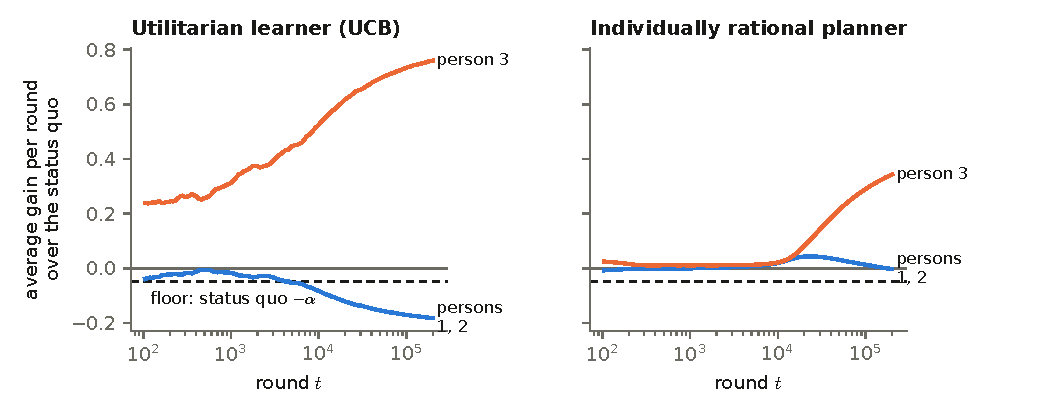
\includegraphics[width=\linewidth]{figures/fig_planner.pdf}
\caption{\Cref{ex:sq}: each person's average gain per round over the status quo, up to round $t$. Left: UCB on the welfare signal finds $\astar$ and takes persons 1 and 2 below the status quo. Right: the individually rational planner of \cref{sec:sq} with $\alpha=0.05$ (mean of 20 runs, band of two standard errors) keeps everyone above the floor and passes most of the gain to person 3.}
\label{fig:planner}
\end{figure}
